\documentclass[border=4pt,class=scrartcl]{standalone}

\usepackage{tikz}
\usetikzlibrary{patterns}
\usetikzlibrary{positioning}
\usetikzlibrary{decorations.pathreplacing}

\begin{document}
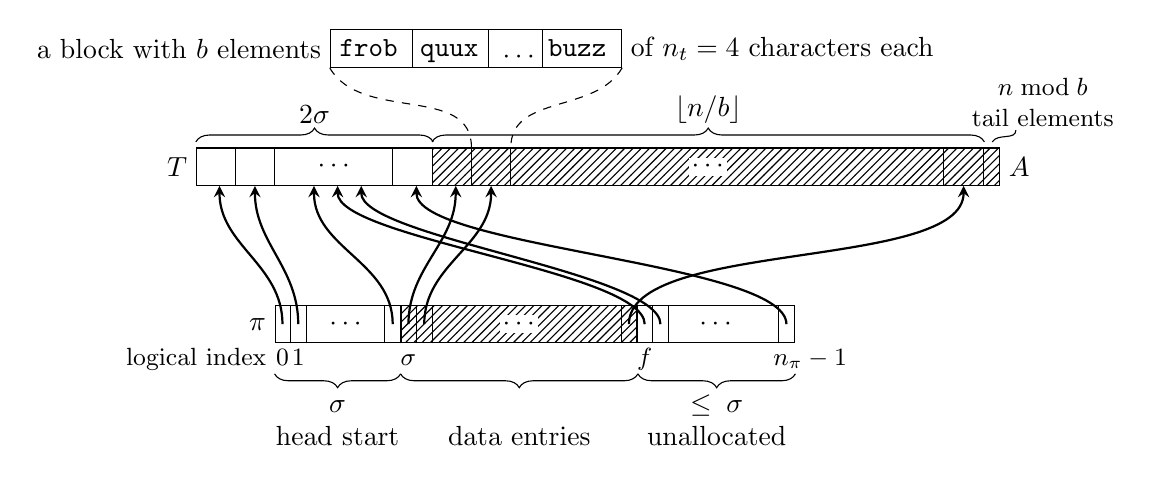
\begin{tikzpicture}


%%  \node at (0,1) {$b = 2$};
%%  \node at (0,.5) {$\sigma = 3 = |\Sigma| = |\{\texttt{a}, \texttt{b}, \texttt{c}\}|$};
%%  \node at (0,0) {$A$};
%%  \node at (-1,0) {$T$};

  %%\node at (-4.2,-.5) {\texttt{---}};
  %%\node at (-3.5,-.5) {\texttt{---}};
  %%\node at (-2.8,-.5) {\texttt{---}};
  %%\node at (-2.1,-.5) {\texttt{---}};
  %%\node at (-1.4,-.5) {\texttt{---}};
  %%\node at (-.7,-.5) {\texttt{---}};
  %%\node at (0,-.5) {\texttt{abc}};
  %%\node at (.7,-.5) {\texttt{bca}};
  %%\node at (1.4,-.5) {\texttt{cab}};
  %%\node at (2.1,-.5) {\texttt{acb}};
  %%\node at (2.8,-.5) {\texttt{bac}};
  %%\node at (3.5,-.5) {$\cdots$};
  %%\node at (4.2,-.5) {\texttt{cba}};
%%
%%  \draw (0,0) rectangle (3,.5);
%%  \draw (3,0) rectangle (10,.5);

  % array T
  \node[draw,minimum width=3cm,anchor=west] at (0,2) (T) {\phantom{A}};
  \node[node distance=-.4pt, left=of T] {$T$};
  \path[draw,decorate,decoration={brace,raise=2pt,amplitude=5pt}]
    (T.north west) -- (T.north east) node[midway,above=5pt]{$2\sigma$};
  \node at (1.75,2) {$\cdots$};
  
  % array A
  \node[draw,minimum width=7.2cm,anchor=west,node distance=-.4pt,right=of T.east,pattern=north east lines, pattern color=black] (A) {\phantom{A}};
  \node[node distance=-.4pt, right=of A] (Alabel){$A$};
  \path[draw,decorate,decoration={brace,raise=2pt,amplitude=5pt}]
    (A.north west) -- ([xshift=-2mm]A.north east) node[midway,above=5pt]  (Anb) {$\lfloor n/b\rfloor$};
  \node[fill=white,inner sep=1pt] at (6.5,2) {$\cdots$};

  % tail of A
  \node[text width=2cm,align=center,font=\small,xshift=3mm,yshift=1mm] at (Alabel |- Anb) {$n\bmod b$\\ tail elements};
  \draw ([xshift=-1mm,yshift=2pt]A.north east) to[out=60,in=270] +(.3,.15);

  
  % array pi  
  \node[draw,minimum width=6.6cm,anchor=west,node distance=-.4pt] at (1,0) (pi) {\phantom{A}};
  \node[node distance=-.4pt, left=of pi] {$\pi$};
  \path[draw,decorate,decoration={brace,raise=11pt,amplitude=5pt,mirror}]
  (pi.south west) -- +(1.6,0) node[midway,below=15pt,text width=2cm,align=center] {$\vphantom\le\sigma$\\ head start};
  \path[draw,decorate,decoration={brace,raise=11pt,amplitude=5pt}]
  (pi.south east) -- +(-2,0) node[midway,below=15pt,text width=2cm,align=center] (f) {$\le\sigma$\\ unallocated};

  \node[draw,fill=black,minimum width=3.0cm,anchor=west,node distance=-.4pt,pattern=north east lines, pattern color=black] at (2.6,0) (data) {\phantom{A}};
  \path[draw,decorate,decoration={brace,raise=11pt,amplitude=5pt}]
  (data.south east) -- (data.south west) node[midway,below=15pt,text width=2cm,align=center] (f) {$\vphantom\le$\\ data entries};

 % indices of pi
 \node[below=-2pt,font=\small,text height=1.5ex,text depth=.25ex] at (1.1,0 |- pi.south) (lindex) {0};
 \node[below=-2pt,font=\small,text height=1.5ex,text depth=.25ex] at (1.3,0 |- pi.south) {1};
 \node[below=-2pt,font=\small,text height=1.5ex,text depth=.25ex] at (2.7,0 |- pi.south) {$\sigma$};
 \node[below=-2pt,font=\small,text height=1.5ex,text depth=.25ex] at (5.7,0 |- pi.south) {$f$};
 \node[below=-2pt,font=\small,text height=1.5ex,text depth=.25ex] at (7.8,0 |- pi.south) {$n_\pi-1$};
  \node[node distance=-3.5pt, left=of lindex,font=\small,text height=1.5ex,text depth=.25ex] {logical index};
  
  % sample block
  \node[draw,minimum width=37mm,anchor=west,node distance=-.4pt] at (1.7,3.5) (sampleblock) {\phantom{A}};
  \node[node distance=-.4pt, left=of sampleblock] {a block with $b$ elements};
  \node[node distance=-.4pt, right=of sampleblock] {of $n_t=4$ characters each};
  \node[anchor=west,text depth=.25ex,text height=1.5ex] at (1.70,3.5) {\texttt{frob}\texttt{~\;quux}};
  \node[text depth=.25ex,text height=1.5ex] at (4.1,3.4) {$\cdots$};
  \node[anchor=west,text depth=.25ex,text height=1.5ex] at (4.35,3.5) {\texttt{buzz}};
\foreach \i in {2.75,3.72,4.4}
\draw (\i,0 |- sampleblock.south) -- (\i,1 |- sampleblock.north);
% zoom the block
\draw[dashed,black] (sampleblock.south west) to[out=300,in=90] (3.5,2 |- A.north);
\draw[dashed,black] (sampleblock.south east) to[out=240,in=90] (4,2 |- A.north);

  
% blocks in T and A
\foreach \i in {0.5,1.0,2.5,3.0,...,4.0,9.5,10}
\draw (\i,0 |- T.south) -- (\i,1 |- T.north);

% entries in pi
\foreach \i in {1.2,1.4,2.4,2.6,...,3.2,5.4,5.6,...,6.2,7.4}
   \draw (\i,0 |- pi.south) -- (\i,1 |- pi.north);


% head start to T
\draw[thick,>=stealth,->] (1.1,0) to[out=90,in=270] (.3,2 |- A.south);
\draw[thick,>=stealth,->] (1.3,0) to[out=90,in=270] (.75,2 |- A.south);
%\draw[thick,>=stealth,->] (1.5,0) to[out=90,in=270] (1.2,2 |- A.south);
\node at (1.9,0) {$\cdots$};
\draw[thick,>=stealth,->] (2.5,0) to[out=90,in=270] (1.5,2 |- A.south);
%%\draw[thick,>=stealth,->] (2.8,0) to[out=90,in=270] (1.5,2 |- A.south);

% data entries to A
\draw[thick,>=stealth,->] (2.7,0) to[out=90,in=270] (3.3,2 |- A.south);
\draw[thick,>=stealth,->] (2.9,0) to[out=90,in=270] (3.75,2 |- A.south);
\node[fill=white,inner sep=1pt] at (4.1,0) {$\cdots$};
\draw[thick,>=stealth,->,looseness=.6] (5.5,0) to[out=90,in=270] (9.75,2 |- A.south);


% free tail to T
\draw[thick,>=stealth,->,looseness=.4] (5.7,0) to[out=90,in=270] (1.8,2 |- A.south);
\draw[thick,>=stealth,->,looseness=.4] (5.9,0) to[out=90,in=270] (2.1,2 |- A.south);
\node at (6.6,0) {$\cdots$};
\draw[thick,>=stealth,->,looseness=.4] (7.5,0) to[out=90,in=270] (2.8,2 |- A.south);


\end{tikzpicture}

\end{document}
